\documentclass[a4paper,12pt,oneside]{book}

%-------------------------------Start of the Preable------------------------------------------------
\usepackage{mathtools}
\usepackage{multicol}
\usepackage[english]{babel}
\usepackage{blindtext}
%packagr for hyperlinks
\usepackage{hyperref}
\hypersetup{
    colorlinks=true,
    linkcolor=blue,
    filecolor=magenta,      
    urlcolor=cyan,
}

\urlstyle{same}
%use of package fancy header
\usepackage{fancyhdr}
\setlength\headheight{26pt}
\fancyhf{}
%\rhead{
\includegraphics[width=1cm]{logo}}
\lhead{\rightmark}
\rhead{
\includegraphics[width=1cm]{logo}}
\fancyfoot[RE, RO]{\thepage}
\fancyfoot[CE, CO]{\href{http://www.e-yantra.org}{www.e-yantra.org}}

\pagestyle{fancy}

%use of package for section title formatting
\usepackage{titlesec}
\titleformat{\chapter}
  {\Large\bfseries} % format
  {}                % label
  {0pt}             % sep
  {\huge}           % before-code
 
%use of package tcolorbox for colorful textbox
\usepackage[most]{tcolorbox}
\tcbset{colback=cyan!5!white,colframe=cyan!75!black,halign title = flush center}

\newtcolorbox{mybox}[1]{colback=cyan!5!white,
colframe=cyan!75!black,fonttitle=\bfseries,
title=\textbf{\Large{#1}}}

%use of package marginnote for notes in margin
\usepackage{marginnote}

%use of packgage watermark for pages
%\usepackage{draftwatermark}
%\SetWatermarkText{
\includegraphics{logo}}
\usepackage[scale=2,opacity=0.1,angle=0]{background}
\backgroundsetup{
contents={
\includegraphics{logo}}
}

%use of newcommand for keywords color
\usepackage{xcolor}
\newcommand{\keyword}[1]{\textcolor{red}{\textbf{#1}}}

%package for inserting pictures
\usepackage{graphicx}

%package for highlighting
\usepackage{color,soul}

%new command for table
\newcommand{\head}[1]{\textnormal{\textbf{#1}}}


%----------------------End of the Preamble---------------------------------------


\begin{document}

%---------------------Title Page------------------------------------------------
\begin{titlepage}
\raggedright
{\Large eYSIP$-$2018\\[1 cm]}
{\Huge\scshape A system for solving jigsaw puzzle using multiple robots\\[.1 in]}
\vfill
\begin{flushright}
{\large Aniket Anantraj Navlur \\}
{\large Kiran Suvas Patil\\}
{\large Ashis Kumar Maharana\\}
{\large Mentor 1$:$ Abinav Sarkar\\}
{\large Mentor 2$:$ Kalind Karia\\}
{\large Duration of Internship: $ 21/05/2018-06/07/2018 $ \\}
\end{flushright}

{\itshape 2018, e-Yantra Publication}
\end{titlepage}
%-------------------------------------------------------------------------------

\chapter[Project Tag]{A System for Solving Jigsaw Puzzle using Multiple Robots}
\section*{Abstract}
The prime motive of this project is to develop a multi Robot based \hspace{0 em} Autonomous Puzzle Solver system that can solve a Jigsaw puzzle.
\section*{Overview of Task}
\begin{tabular}{| c | p{27 em} | }\hline
		\textbf{Task No.} & \hspace{10 em}\textbf{Task}\\\hline
		1 &\small{ Python, OpenCV, Firebird V Intro,XBee Communication} \\\hline
		2 &\small{ Pose and orientation calculation of 2 Firebird robots using\hspace{3 em} color/Aruco markers }\\\hline
		3 &\small{ Programming the Go-To-Goal Controller for single Firebird V robot. Tuning the PID\hspace{0 em} values to perfection }\\\hline
		4 &\small{ Implementing path planning with Firebird V where obstacles have been placed in arena }\\\hline
		5 &\small{ Detection of jigsaw puzzle blocks using\hspace{0 em}Template Matching}\\\hline
		6 &\small{ Pick and place of blocks - gripper mechanism building }\\\hline
		7 &\small{ Implementing the entire solution for a given\hspace{0 em}jigsaw puzzle }\\\hline
		8 &\small{ Documentation and reporting results }\\\hline
	\end{tabular}

\subsection*{Completion status}
We have successfully implemented the theme and completed all the deliverables. Whole of the solution is successfully implemented using a single robot with good efficiency. The theme is also implemented using multiple robots, but the efficiency is around 50\% for obstacle avoidance.  

\section{Hardware parts}
\begin{itemize}
  \item FireBird Robots(2)
  \item  XBee(3)
  \begin{itemize}
  \item Xbee module
  \item Xbee usb adapter board
  \item USB type B to type A converter
  \end{itemize}
   \item Overhead Camera
   \item ArUco markers
   \item Servo motors for gripper mechanism
   \item Flex sheet for arena
   \item Puzzle pieces
\end{itemize}

\section{Software used}
\begin{itemize}
  \item Python
  \item OpenCV
  \item AVR Studio 5.1
  \item XCTU(latest version)
  \item AVRDude
  \item Fusion360
\end{itemize}
\section{Hardware Design}
\subsection*{Gripper Mechanism}
The gripper mechanism is build for a bigger block size $12cm\times{12cm\times{12cm}}$. Alongside the gripper we need two more degrees of freedom. One for picking the block and another for rotating the block. As the block has to be rotated around its z-axis we are picking it from top. That makes the gripper to be placed at a height higher than $12cm$. And the servo that will rotate the block has to be placed higher than that and at some
distance such that while rotating or opening the gripper, it should not touch the robot in order not to damage the gripper. We are using dual shaft servos and their brackets. Once the platform and arm is made we went for some inspiration from the internet for the gripper and tried simulating different ones. Then we finished with a simpler one not to make it heavy for the arm and servo. Once designed in $Fusion360$  and tested in simulation, we 3D printed the prototype. Once satisfied with the performance we printed two more of them for two robots. For a good grip we made the gripping plates wider and are using rubber bands and foam. By changing the gripping angle it can pick a block as big as $12cm$.\\
The final gripper that is designed is given below. All these parts are designed in \textbf{Fusion 360} with proper measurements and 3D printed.
\begin{center}
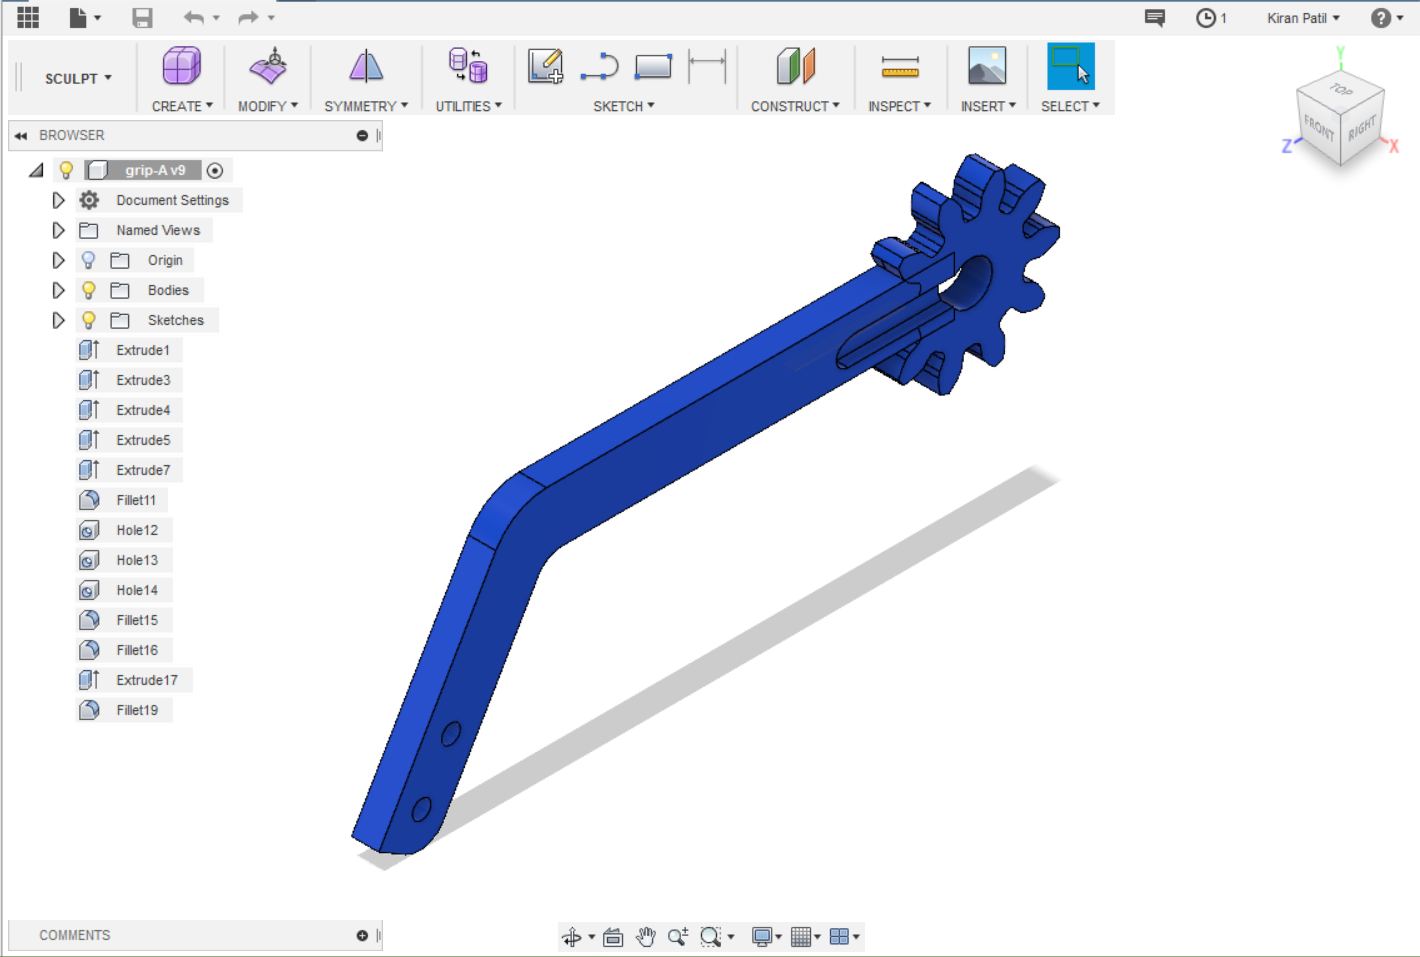
\includegraphics[scale=0.2]{gear1.png}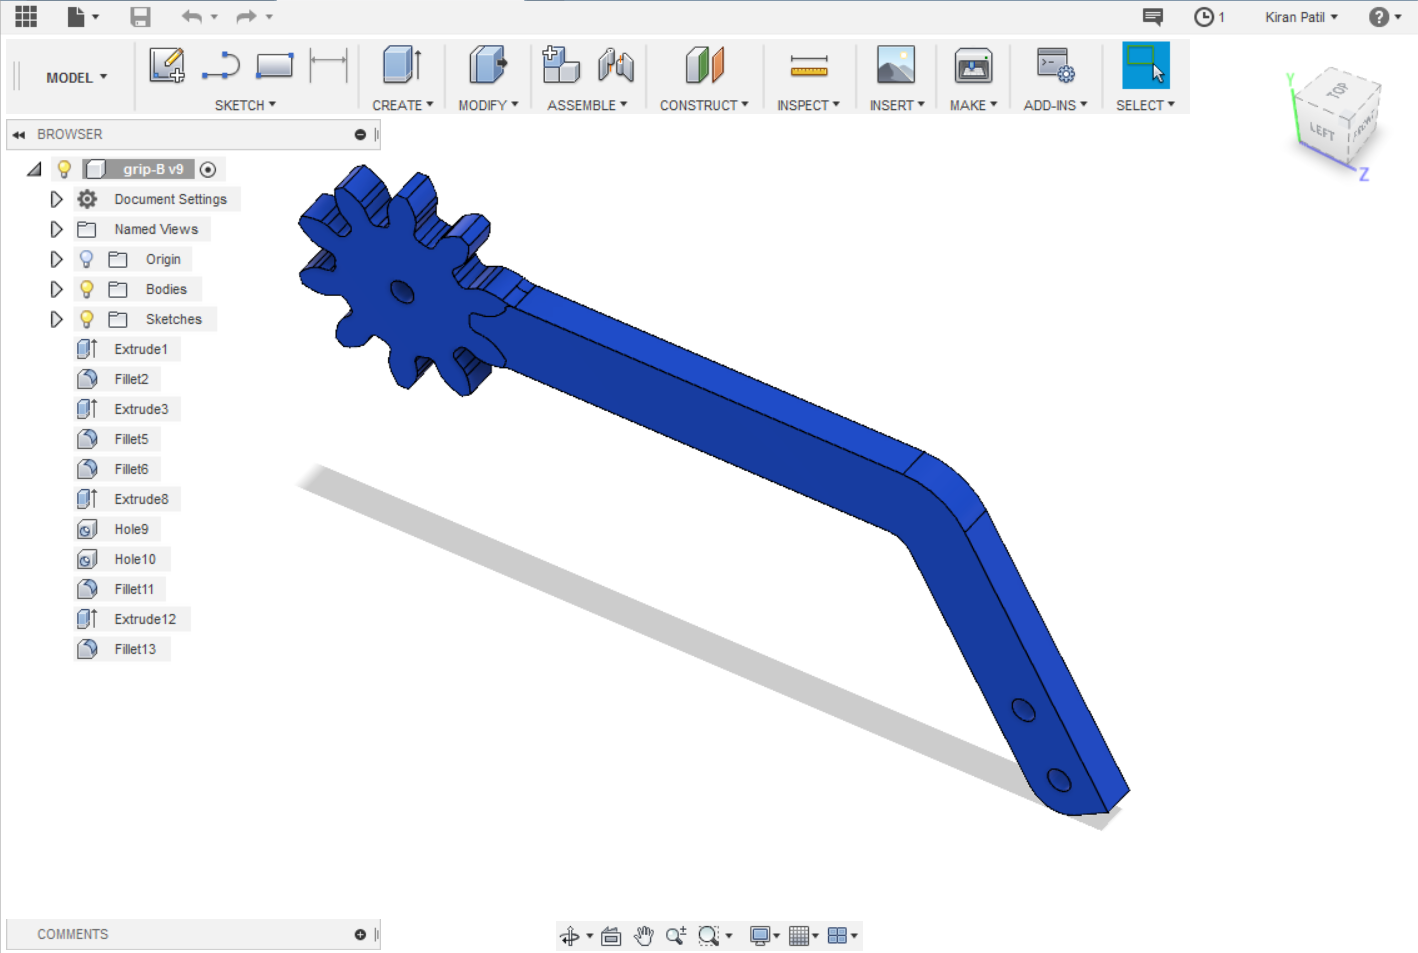
\includegraphics[scale=0.2]{gear2.png}\\
\small{Figure\textbf{. Right Gear} \hspace{5 em}Figure\textbf{. Left Gear}}
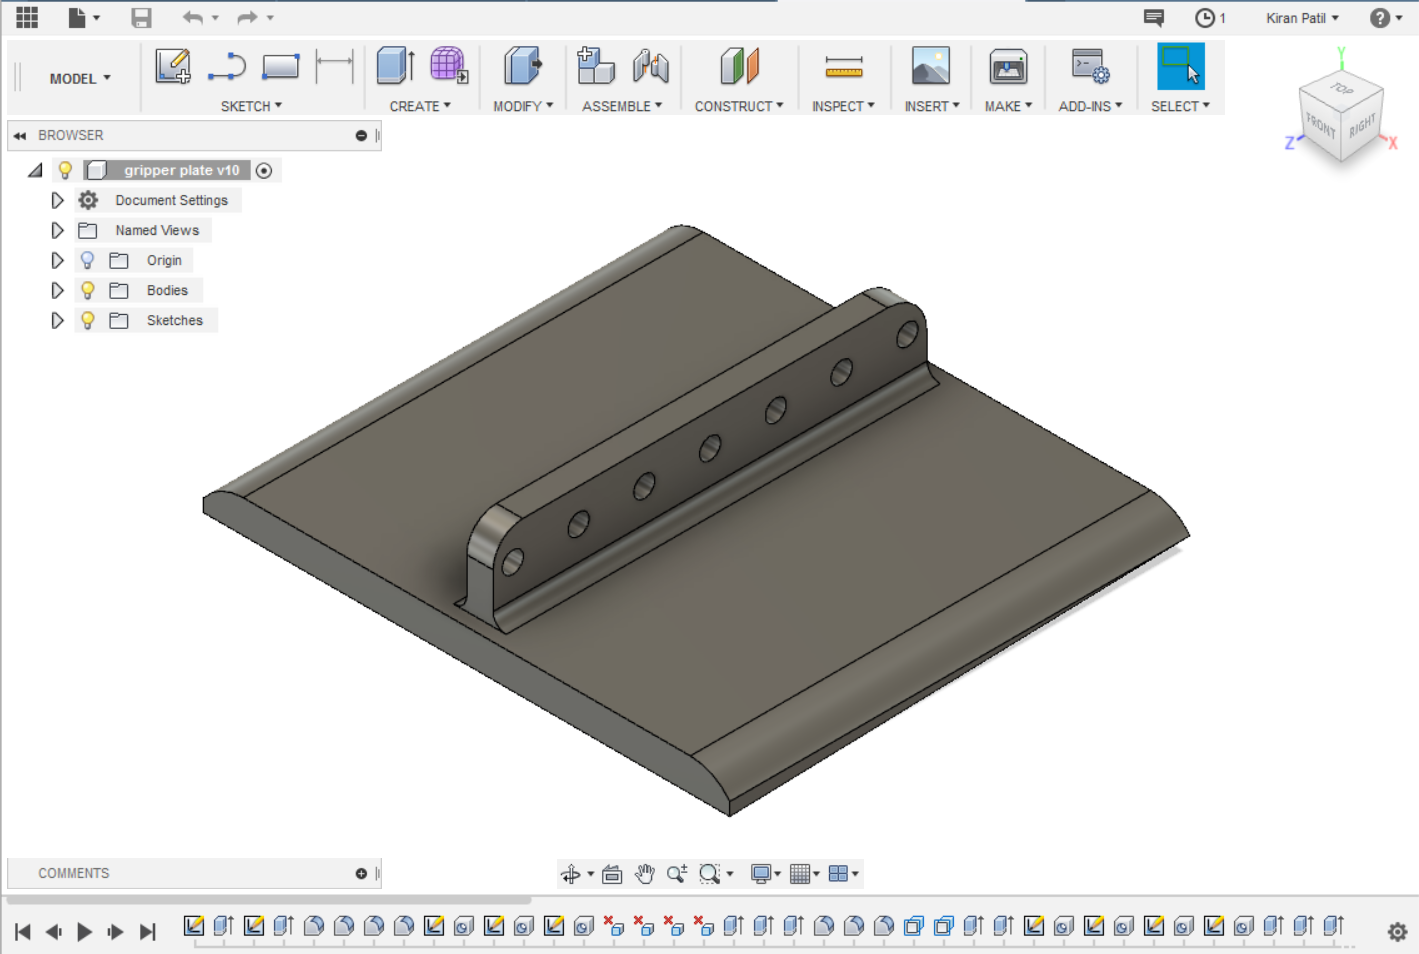
\includegraphics[scale=0.2]{gripplate.png}
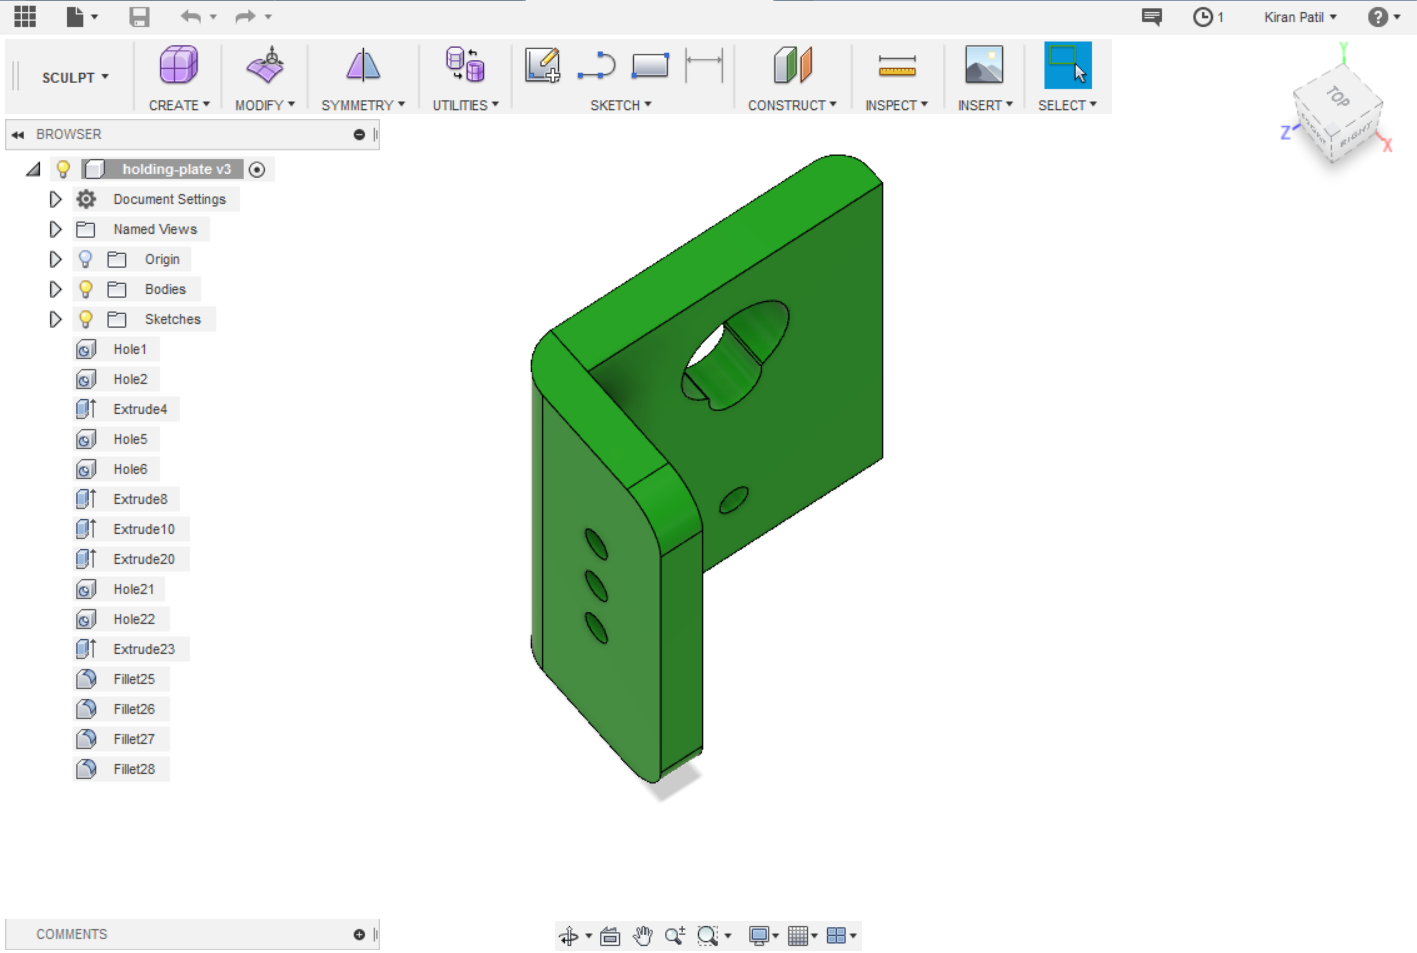
\includegraphics[scale=0.2]{HoldingPlate.png}\\
\small{Figure\textbf{. Gripping Plate} \hspace{5 em}Figure\textbf{. Servo Holder}}\\
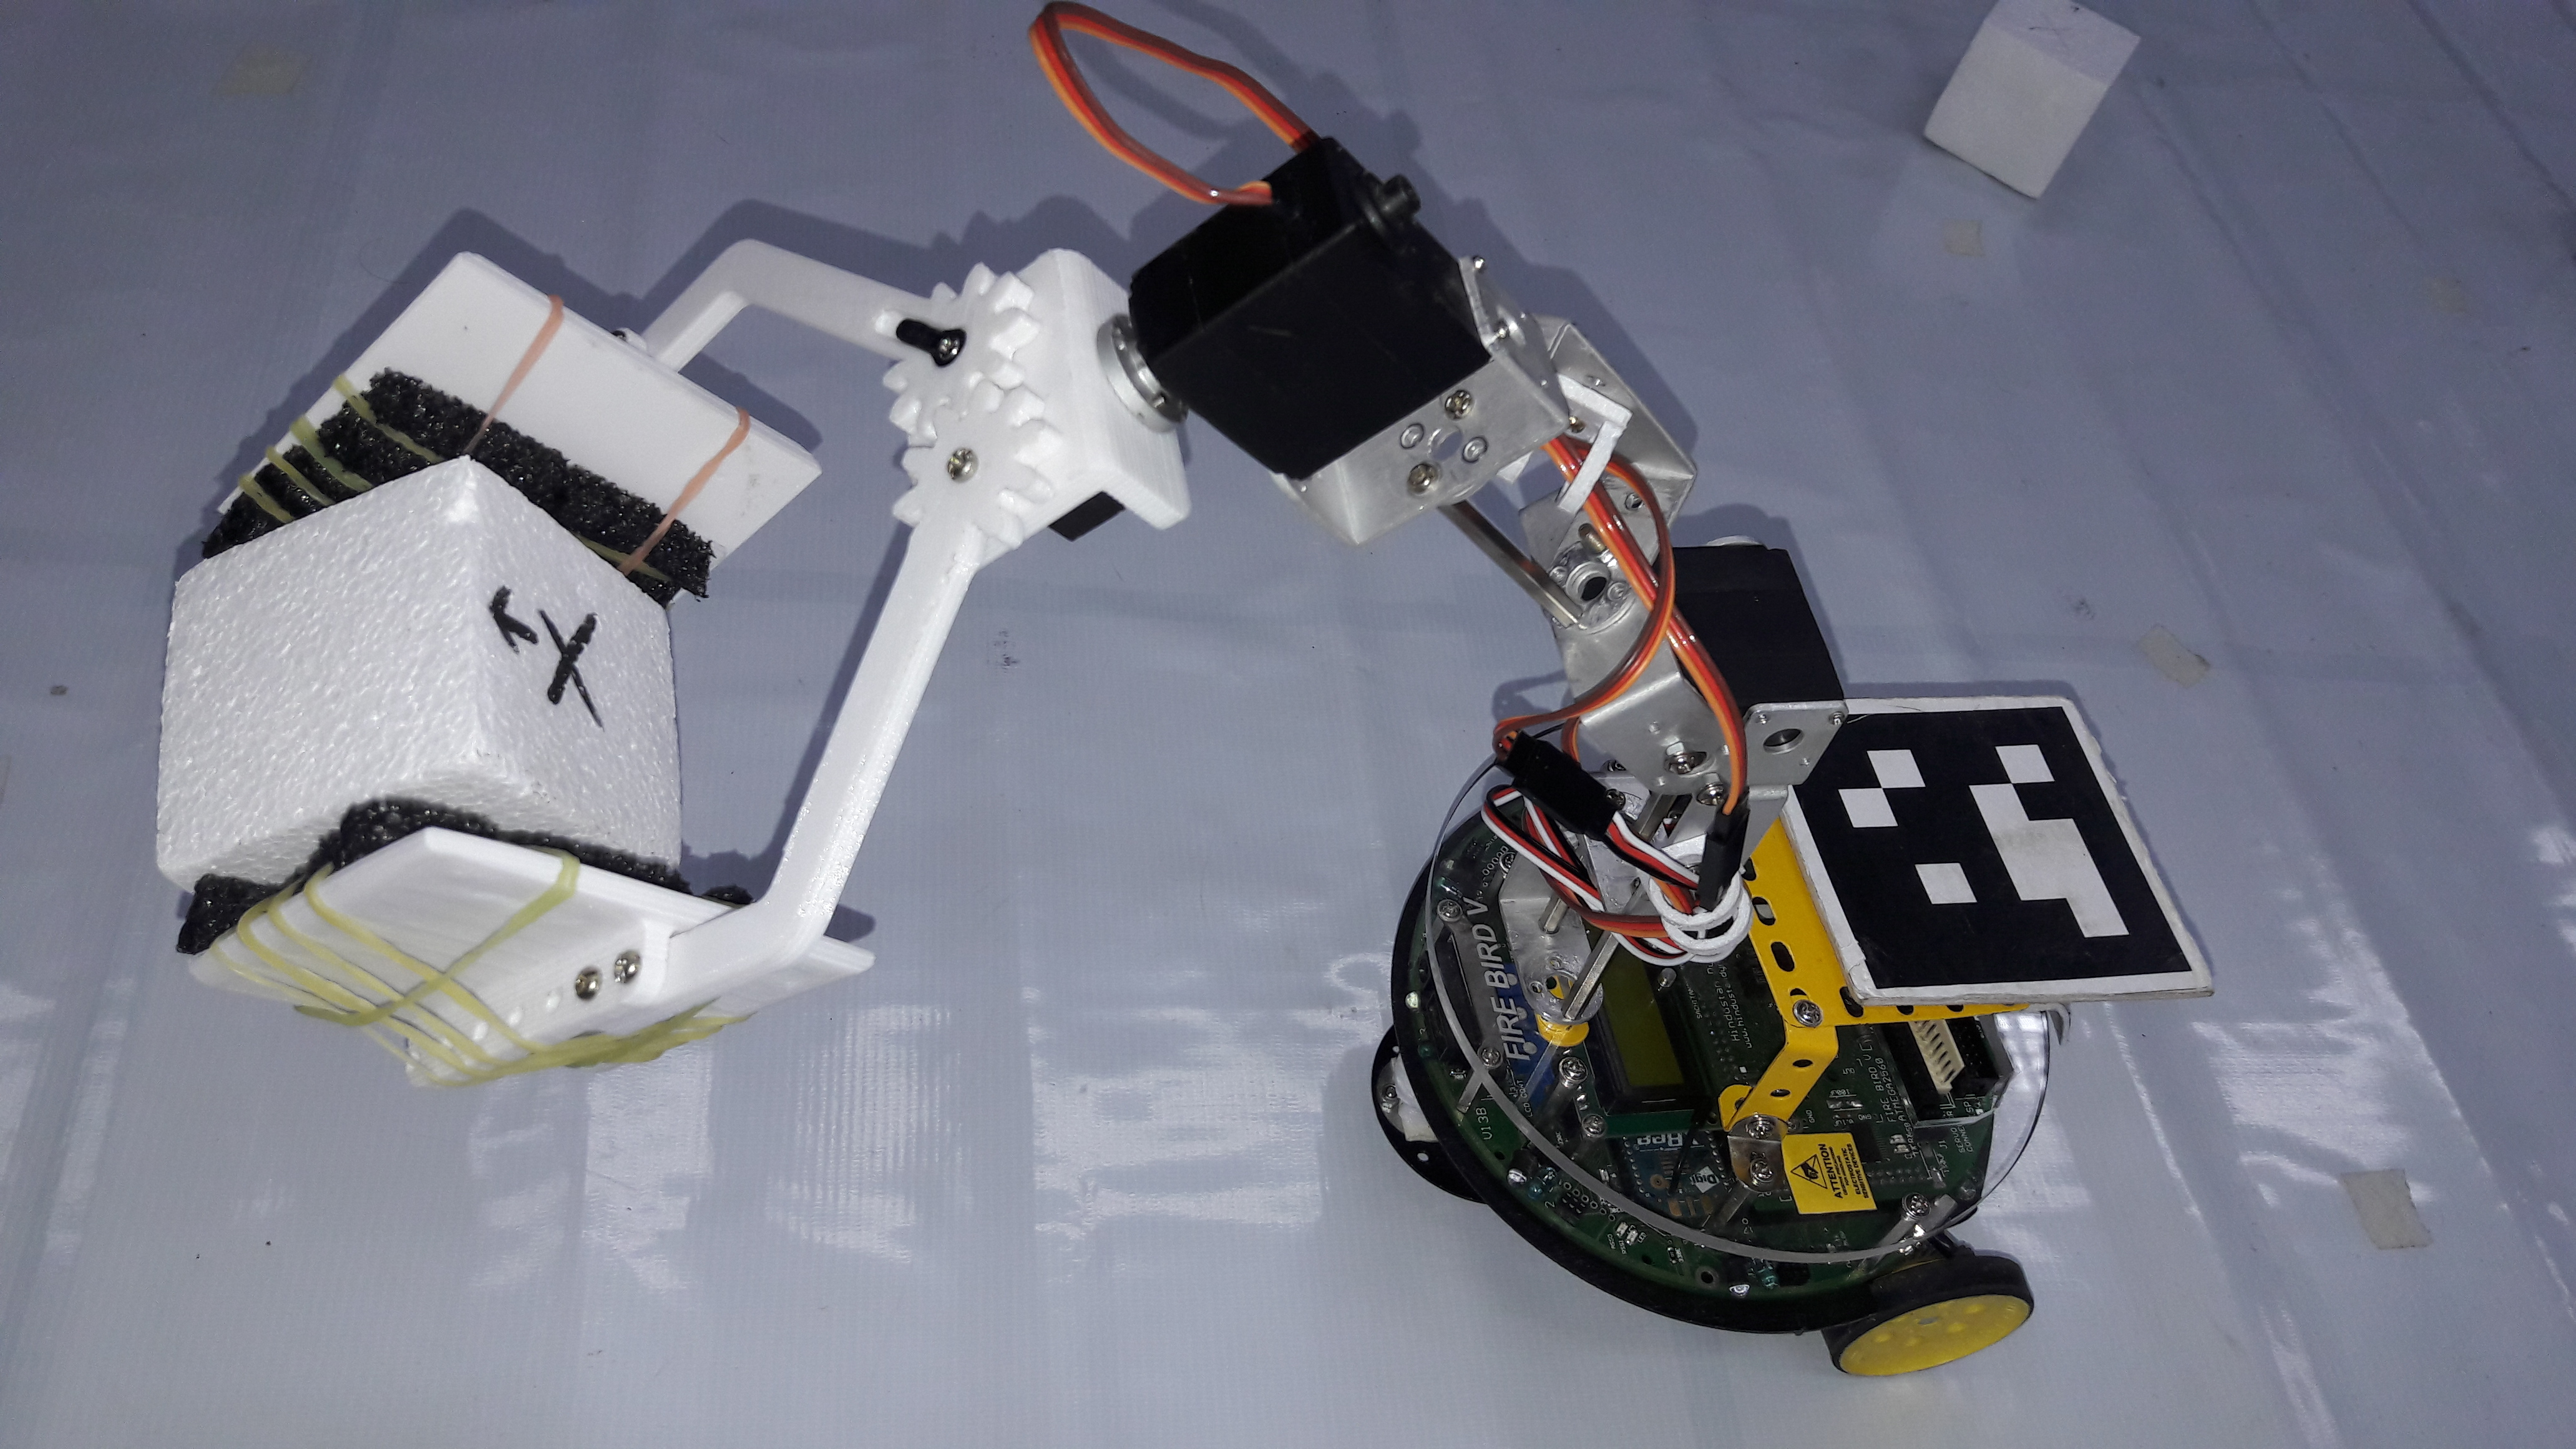
\includegraphics[scale=0.045]{final.jpg}\\
\small{Figure\textbf{. Final assembled arm and gripper}}
\end{center}
\section{Software and Code}
\subsection*{Dependencies}
Before configuring the XBee modules one should first understand the different parameters of it. This article\textsuperscript{1} should help.  For configuring the xbee modules latest XCTU software is used. The channel is chosen so, such that no other device interfere the communication. 
\subsubsection*{$>>$ArUco module}
Detection of ArUco markers using python requires integration of aruco library to the current python version installed. The aruco library can be found in opencv-contrib module. For installing opencv-contrib follow these \href{https://www.youtube.com/watch?v=jnpC_Ib_lbc}{steps\textsuperscript{2} }$($ installing modules using pip $)$. 
\begin{center} 
\framebox{\textcolor{gray}{ pip install opencv-contrib-python }}
\end{center}
\subsubsection*{$>>$Set up for Communication}
For communicating to xbee module using python requires xbee and pyserial module. There are many similar modules for serial communication and xbee, but we need these two modules. One can search and go through other modules also. One is given below.
\begin{enumerate}
\item \href{https://pypi.org/project/pyserial/}{pyserial\textsuperscript{3}}
\begin{center} 
\framebox{\textcolor{gray}{ pip install pyserial }}
\end{center}
\item \href{https://pypi.org/project/XBee/}{xbee\textsuperscript{4}}
\begin{center}
\framebox{\textcolor{gray}{ pip install xbee }}
\end{center}
\item optional \href{https://pypi.org/project/digi-xbee/}{digi-xbee\textsuperscript{5}}
\begin{center}
\fbox{\textcolor{gray}{ pip install digi-xbee }}
\end{center}
\end{enumerate}\vspace{0 em}
The xbee model provided(XBee S2C) cannot be read properly using the earlier versions of XCTU. So it is recommended to use the \href{https://www.digi.com/support/productdetail?pid=3352&type=utilities}{latest version\textsuperscript{6}}. Follow the previous Docs for configuration using XCTU. After configuration and testing over XCTU, communication is again tested using the python script. Once the communication is established it is time to connect the xbee modules on the Firebird V robots. How to guide can be found in the hardware manual of Firebird V.
\subsubsection*{$>>$Image rotation}
For rotating the image in case of template matching we are using rotate function available in imutils module. To install \href{https://www.pyimagesearch.com/2015/02/02/just-open-sourced-personal-imutils-package-series-opencv-convenience-functions/}{imutils\textsuperscript{7}}
\begin{center}
\framebox{\textcolor{gray}{pip install imutils}}
\end{center}
\subsection*{ArUco detection}
Then comes the localisation of robots. For that purpose we are using overhead camera and ArUco markers. The position and orientation of the ArUco marker is first calculated using python script and \href{https://docs.python.org/2/library/math.html}{math module\textsuperscript{8}} which is inbuilt in python. Angle is calculated such that it ranges from 0 to 360 degrees. The python script can be found \href{https://github.com/eYSIP-2018/Jigsaw_Puzzle_Solver_using_Multiple_Robots/blob/master/Scripts/ArUco detection orientation/Aruco_pose.py}{here}.
\begin{center}
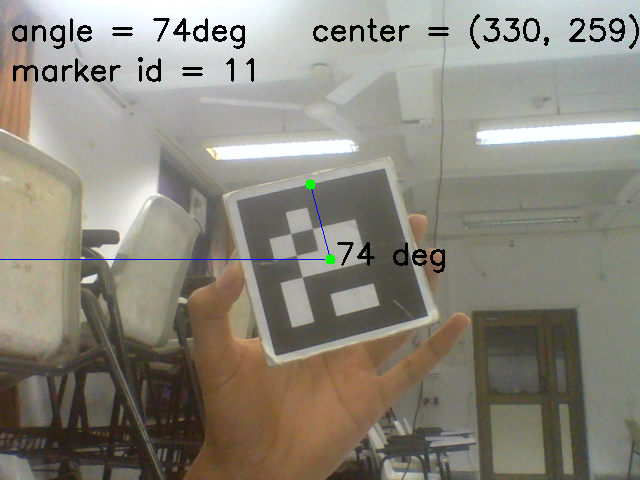
\includegraphics[scale=0.5]{aruco.png}\\
\small{Figure\textbf{. ArUco orientation and position}}
\end{center}
\subsection*{Go-To-Goal Controller}
For the Go-To-Goal Controller we first found the orientation and distance of the robot from its goal or destination. Then the error angle is calculated by subtracting angle with respect to frame from angle with respect to destination. The code can be found \href{https://github.com/eYSIP-2018/Jigsaw_Puzzle_Solver_using_Multiple_Robots/blob/master/Scripts/ArUco detection orientation/Aruco_pose_with_other_point.py}{here}. In another way the error angle can be found by
\begin{center}
$error angle = \arctan \left (\frac{m - n}{1 - m\times n}\right)$\\
m = orientation of robot with respect to frame\\
\hspace{2.7 em}n = orientation of robot with respect to destination\end{center}
This error angle is then passed to the PID controller which then adjusts the speed of motors to maintain a zero error. The python script sends data packets to the Firebird V robot via Xbee. These data packets are formed by the following values.
\begin{center}
\includegraphics[scale=0.5]{capture.png}\\
\small{Figure\textbf{. Packet example}}\\
$\left\langle T|d_x|d_y|P|K_p|K_i|K_d|R|r_x|r_y|A|angle |\right\rangle$\\
$<$ symbolizes beginning of data packet\\
T symbolizes target\\
d\textsubscript{x} $=$ destination x co-ordinate\\
d\textsubscript{y} $=$ destination y co-ordinate\\
P symbolizes PID gains\\
K\textsubscript{p} $=$ proportional gain\\
K\textsubscript{i} $=$ integral gain\\
K\textsubscript{d} $=$ differential gain\\
R symbolizes robot position\\
r\textsubscript{x} $=$ robot x co-ordinate\\
r\textsubscript{y} $=$ robot y co-ordinate\\
A symbolizes error angle\\
$>$ symbolizes end of packet\end{center}
Once received, the packet is successfully parsed by the robot in an ISR and the speeds are assigned to the motors as PWM duty-cycle.The \href{https://github.com/eYSIP-2018/Jigsaw_Puzzle_Solver_using_Multiple_Robots/blob/master/Firebird V/firebird.c}{c code} and python \href{https://github.com/eYSIP-2018/Jigsaw_Puzzle_Solver_using_Multiple_Robots/tree/master/Scripts/PID control}{script} can be found here. When the robot is around 10 pixels away from its destination it stops, showing it has reached the destination. This is because the robot is bigger then the marker and before the center point reaches its destination robot will have already reached there.
We completed the path planning in various steps. When the destination is given to the python script it first determines which of the two robots is nearer to the destination and then it sends packets to that robot. Video can be found \href{https://youtu.be/o74QrQ3lfsw}{here}.
\subsection*{Path planning with Obstacle avoidance}
The next step is to avoid obstacles. For a robot moving towards its destination, the other robot and the puzzle blocks except the one at its destination are the obstacles for the robot. One of the obstacles is a moving one so the obstacle map needs to be dynamic. So we have to build the obstacle map in every frame. And the path finding algorithm should be fast enough too. We tried various algorithms like dijkstra's\textsuperscript{[10]} with voronoi\textsuperscript{[9]}, Lee's, A*\textsuperscript{[11]} and finally concluded with A* algorithm which seemed fast and reliable. The center points of the obstacles are given to a function which then draws a rectangle around it. The area of the rectangle is treated as the obstacle. So the path finding algorithm avoids those rectangles. We have taken care of the size of the robot by drawing circle around the center of the robot. The path is planned such that there is some distance between the robot's outer shell and the obstacle. Robot's body should not touch the obstacle. First it is done for a single robot then it is implemented for a multi robot environment. Link to the code is given. Video can be found \href{}{here}.
\subsection*{Template Matching}
For solving a jigsaw puzzle we first have to determine which puzzle block goes where. This is done by template matching. We are given with the static image of the arena where there are puzzle blocks placed with different orientation and the final image we have to make out of those puzzle blocks. We first detect the puzzle block from the arena and separate it from background. The final image is divided into same number of pieces as present in the arena. We number each of the piece according to their position. Then we run a template matching function which rotate the block obtained from the arena by 1 degree and finds percentage matching with every piece of final image. For which number piece the matching percentage is maximum, is then
assigned to the block along with the angle that gave the maximum match. The code can be found \href{https://github.com/eYSIP-2018/Jigsaw_Puzzle_Solver_using_Multiple_Robots/blob/master/Scripts/arena and puzzle block detection/input_output.py}{here}. This angle and robot's orientation both play major role in picking and placing the puzzle block at its destination.
\begin{center}
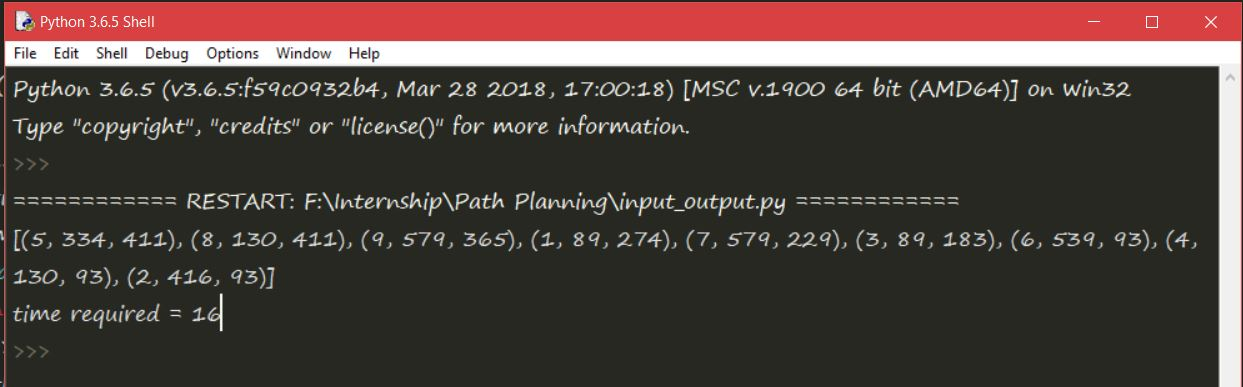
\includegraphics[scale = 0.35]{templatem.jpg}\\
\small{Figure\textbf{. Puzzle block no. and block position}}\\
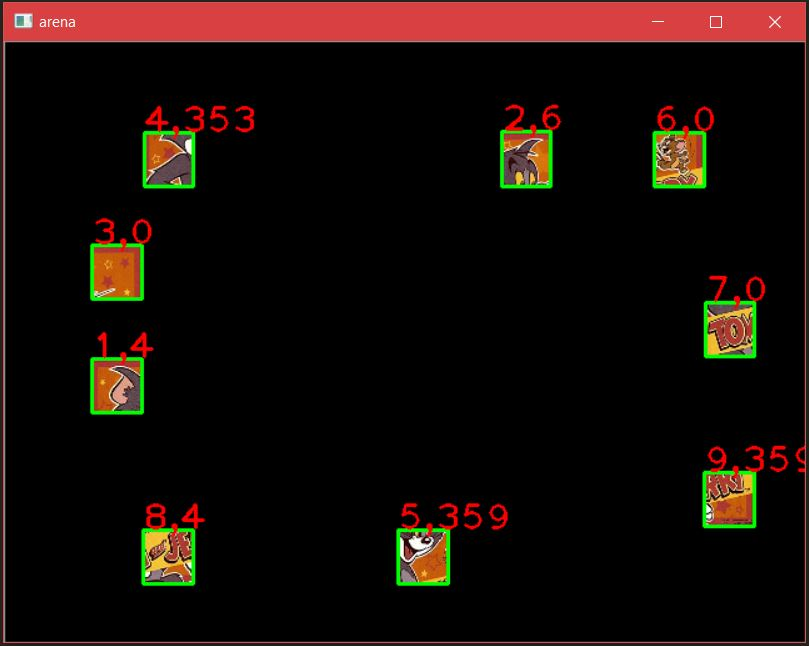
\includegraphics[scale = 0.4]{template.jpg}\\
\small{Figure\textbf{. Puzzle block no. and orientation obtained from Template matching}}\\
\end{center}

\subsection*{Final Implementation}
The whole of the solution is first implemented for a single robot. Every block has 4 pickup points around it and at the center there is a point assigned where it will be placed and where the robot has to be to place it correctly. The path finding algorithm finds the nearest point out of those 4 point for the nearest block and goes there. Once reached it then aligns parallel to the side of block it is facing. It then rotates the gripper if needed and picks the block, travel to the destination for that particular block avoiding all other blocks, place it in proper orientation and then moves towards next nearest block. Here is the \href{https://github.com/eYSIP-2018/Jigsaw_Puzzle_Solver_using_Multiple_Robots}{link} to codes.
\section{Flowcharts}

\section{Demo}
Here are the links of demonstration video.
\begin{itemize}
\item \href{https://youtu.be/_RwL_YZDmpI}{link} for single robot demo
\item \href{https://youtu.be/jv9p9h0FJP0}{link} for multi robot demo
\end{itemize} 

\section{Future Work}
A multi robot box pushing problem can be implemented by tweaking some of the functions and using complex mathematics. Instead of avoiding collision between robots, they should pass the blocks to the other one when they come near.
\section{Bug report and Challenges}
\begin{itemize}
\color{red}
\item ArUco orientation\\\color{black}
The math module and the math header file in python and c respectively includes $arctan$, but for slope greater than -1 and less than 1 it does not give any output. We are unable to get the the angles between -45 and 45. So we went for $arccot$ for this range then converted it back into $arctan$. So we are calculating the angle and sending it to the robot instead of letting it calculate.
\color{red}
\item Block size\\\color{black}
When building the obstacle map it is taken care that the two robots do not collide.
\color{red}
\item Gripper\\\color{black}
The gripper mechanism needs to be light and big enough to pick and place a big size block. Light because it should not add extra weight to the servo.
\color{red}
\item Moving obstacle\\\color{black}
Path planning has to be done avoiding the moving obstacle.
\color{red}
\item Power to drive the servos\\\color{black}
While testing we found that the servo driver could not provide that much power to drive the servos. So we tried shutting all the sensors and LCD which helped a little.
\color{red}
\item Camera\\\color{black}
The frame captured from the camera should be big enough to accommodate all the blocks and two robots and also focus should be good for the markers to be detected properly everywhere. 
\end{itemize}


\begin{thebibliography}{li}
\bibitem{XCTU}
{Exploring xbees and xctu}\\
${https://learn.sparkfun.com/tutorials/exploring-xbees-and-xctu}$

\bibitem{pip}
{installing modules using pip}\\
$https://www.youtube.com/watch?v=jnpC_Ib_lbc$
\bibitem{pyserial}
{pyserial library}\\
$https://pypi.org/project/pyserial/$

\bibitem{XBee}
{XBee library}\\
$https://pypi.org/project/XBee/$

\bibitem{digi-xbee}
{digi-xbee library}\\
$https://pypi.org/project/digi-xbee/$

\bibitem{xctu latest}
{Download link }XCTU latest version\\
$https://www.digi.com/support/productdetail?pid=3352\&type=utilities$
\bibitem{imutils}
{imutils library}\\
$https://www.pyimagesearch.com/2015/02/02/just-open-sourced-personal-imutils-package-series-opencv-convenience-functions/$

\bibitem{math}
{math library}\\
$https://docs.python.org/2/library/math.html$

\bibitem{3D}
Gripper Design inspiration\\
$https://www.thingiverse.com/search?q=gripper+arm\&dwh=985b3b60dfeacfe$
\bibitem{voronoi}
{voronoi}\\
$https://docs.scipy.org/doc/scipy/reference/spatial.html$
\bibitem{dijkstra's}
{Dijkstra's algorithm}\\
$https://gist.github.com/econchick/4666413$
\bibitem{A*}
{A* path finding algorithm explanation}\\
$https://www.youtube.com/watch?v=aKYlikFAV4k\&t=1429s$
\bibitem{A* code}
{A* path finding algorithm python}\\
$http://code.activestate.com/recipes/578919-python-a-pathfinding-with-binary-heap/$

\end{thebibliography}
\end{document}

